% ============================================================
%  GUÍA 2: NÚMEROS ENTEROS Y SUS OPERACIONES
%  Curso Introductorio de Matemáticas — 1er Año
%  Autor: Ing. Gabriel Astudillo
%  Sesiones cubiertas: Semana 2 (clases 5 a 8)
% ============================================================

\documentclass[12pt, a4paper]{article}

% ── Paquetes ─────────────────────────────────────────────────

\usepackage{mathwizards-guia}
\mwguia{Guía 2 — Números Enteros y sus Operaciones}{Ing. Gabriel Astudillo $\cdot$ Curso 1er Año}

% ── Comandos propios de esta guía ───────────────────
\newcommand{\Z}{\mathbb{Z}}

\begin{document}
% ============================================================

% ── Portada / Título ─────────────────────────────────────────
\mwportada{Guía de Estudio 2}{Los Números Enteros y sus Operaciones}{Suma, Resta, Multiplicación, División y Operaciones Combinadas en $\Z$}

\vspace{4pt}
\begin{cuadroinfo}
  \small
  \textbf{Presentación:} \textquestiondown Sabías que hay números \emph{por debajo de cero}? Los usamos todos los días: cuando hace frío en la sierra ($-3\,^{\circ}$C), cuando el ascensor baja a un sótano (piso $-2$) o cuando debes dinero en una alcancía ($-15$ Bs.). Esos números se llaman \textbf{enteros negativos}, y en esta guía aprenderás a operar con ellos como un verdadero experto. También descubrirás la famosa \emph{regla de los signos} y el orden correcto para hacer operaciones combinadas.
  \\[4pt]
  \textbf{Nivel de Dificultad:}\quad
  \facil{} Básico / Directo \quad
  \medio{} Intermedio \quad
  \dificil{} Desafiante
\end{cuadroinfo}

\vspace{8pt}

% ============================================================
\section{Suma y Resta de Números Enteros}
% ============================================================

\subsection{\textquestiondown Qué es el conjunto de los enteros?}

El conjunto de los \textbf{números enteros} (que se escribe $\Z$) está formado por:

\begin{cuadroteoria}
  \textbf{Definición:}
  \[
    \Z = \{ \dots, -3, -2, -1, 0, 1, 2, 3, \dots \}
  \]
  \begin{itemize}
    \item Los números \textbf{positivos} ($1, 2, 3, \dots$) están a la derecha del cero.
    \item Los números \textbf{negativos} ($-1, -2, -3, \dots$) están a la izquierda del cero.
    \item El \textbf{cero} ($0$) no es positivo ni negativo: es el punto de partida.
  \end{itemize}
\end{cuadroteoria}

\noindent Podemos dibujarlos en la \textbf{recta numérica}, una recta donde cada número tiene su casita:

\begin{center}
  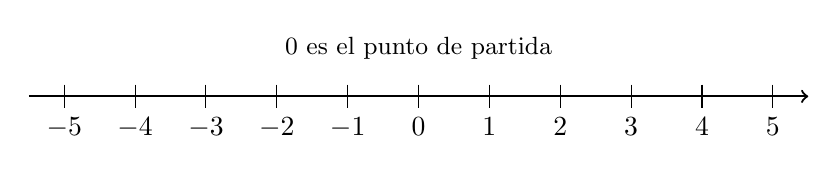
\begin{tikzpicture}[x=0.9cm]
    \draw[->, thick] (-5.5,0) -- (5.5,0) node[below left] {};
    \foreach \x in {-5,-4,...,5} {
        \draw (\x,0.15) -- (\x,-0.15) node[below] {$\x$};
      }
    \node[above] at (0,0.35) {\small $0$ es el punto de partida};
  \end{tikzpicture}
\end{center}

\noindent Caminar a la \textbf{derecha} es sumar; caminar a la \textbf{izquierda} es restar. Por ejemplo, para calcular $-3 + 5$: partimos de $-3$ y damos $5$ pasos a la derecha... llegamos a $2$.

\subsection{El valor absoluto}

\begin{cuadroteoria}
  \textbf{Definición:} el \textbf{valor absoluto} de un número entero $a$ se escribe $|a|$ y es \emph{la distancia} desde $a$ hasta el cero en la recta. La distancia siempre es positiva o cero.

  Ejemplos: $|5| = 5$, $|-5| = 5$, $|0| = 0$.
\end{cuadroteoria}

\noindent Los números $-5$ y $5$ están a la misma distancia del cero, por eso $|-5| = |5| = 5$.

\subsection{Regla de los signos para sumar y restar}

\begin{cuadrosolucion}
  \textbf{Para sumas y restas:}
  \begin{itemize}
    \item \textbf{Igual signo:} suma los números y conserva el signo.
          \quad $-4 + (-3) = -7$ \quad y \quad $5 + 8 = 13$.
    \item \textbf{Signos diferentes:} resta el número con mayor valor absoluto menos el otro, y colocarás el signo del número más grande de los dos (con mayor valor absoluto)
          \quad $-7 + 4 = -3$ \quad y \quad $7 + (-4) = 3$.
  \end{itemize}
\end{cuadrosolucion}

%\begin{cuadrosolucion}
%  \textbf{Para restar:} restar un número es lo mismo que \textbf{sumar su opuesto}:
%  \[
%    a - b = a + (-b)
%  \]
%  Ejemplo: $5 - 9 = 5 + (-9) = -4$. \quad Ejemplo: $-3 - 4 = -3 + (-4) = -7$.
%\end{cuadrosolucion}

\begin{cuadroadvertencia}
  \textbf{Los signos dobles:} cuando aparecen dos signos juntos, los resolvemos así:
  \[
    + (+) = + \qquad +(-) = - \qquad -(+) = - \qquad -(-) = +
  \]
  Ejemplo: $8 - (-3) = 8 + 3 = 11$. \quad Ejemplo: $-5 + (-2) = -5 - 2 = -7$.
\end{cuadroadvertencia}

\noindent\textbf{Ejemplo resuelto:} La temperatura en la mañana era de $-4\,^{\circ}$C y subió $10\,^{\circ}$C. \textquestiondown Cuál es la nueva temperatura?

\[
  -4 + 10 = 6
\]

\noindent La nueva temperatura es $6\,^{\circ}$C.

\subsection{Ejercicios: Suma y Resta en $\Z$}

\begin{enumerate}[leftmargin=*]
  \item \facil{} $-3 + 5$

  \item \facil{} $7 + (-2)$

  \item \facil{} $-4 + (-3)$

  \item \facil{} $-8 + 8$

  \item \facil{} $6 + 9$

  \item \facil{} $0 + (-5)$

  \item \medio{} $-12 + 7$

  \item \medio{} $5 - 9$

  \item \medio{} $-3 - 4$

  \item \medio{} $-6 + 6 + (-6)$

  \item \medio{} $10 - 17$

  \item \medio{} $-9 - (-3)$

  \item \medio{} $-5 + 5 - 5$

  \item \medio{} En la sierra la temperatura era de $-4\,^{\circ}$C y subió $10\,^{\circ}$C. \textquestiondown Cuál es la nueva temperatura?

  \item \medio{} Mario le debe $15$ Bs. a su hermana y hoy le paga $8$ Bs. \textquestiondown Cuánto le debe todavía? (Escríbelo como un número entero.)

  \item \dificil{} $-2 + 7 - 9 + 3$

  \item \dificil{} $8 - 12 + 5 - 1$

  \item \dificil{} Un ascensor está en el piso $5$. Baja $7$ pisos, sube $3$ y baja $4$. \textquestiondown En qué piso queda?

  \item \dificil{} Completa con $+$ o $-$ para que la igualdad sea verdadera:
        \begin{enumerate}[label=\alph*)]
          \item $(-5) \ \_\_ \ (-3) = -8$
          \item $(-5) \ \_\_ \ (-3) = -2$
        \end{enumerate}

  \item \dificil{} \textbf{El reto de los campeones:} Pienso un número entero, le sumo $-7$ y obtengo $-2$. \textquestiondown Cuál es el número? (Trabaja hacia atrás.)
\end{enumerate}

\newpage

% ============================================================
\section{Multiplicación y División de Números Enteros}
% ============================================================

\subsection{La regla de los signos}

Multiplicar es sumar repetido. Por ejemplo, $3 \times (-2)$ significa \emph{tres veces perder $2$}: $(-2) + (-2) + (-2) = -6$. Y multiplicar dos negativos... \textquestiondown sabías que da positivo? Piensa en la doble negación: \emph{«no es cierto que no tengo deudas»} significa que sí tengo deudas... no, espera: \emph{«no es cierto que no gané»} significa que sí gané. ¡Dos negativos se anulan!

\begin{cuadroteoria}
  \textbf{Regla de los signos (multiplicación y división):}
  \[
    \begin{array}{c|c|c}
      \text{signo} & \text{signo} & \text{resultado} \\ \hline
      +            & \times       & +                \\[2pt]
      +            & \times       & -                \\[2pt]
      -            & \times       & +                \\[2pt]
      -            & \times       & -                \\[2pt]
    \end{array}
  \]
  \noindent En palabras:
  \begin{itemize}
    \item $+ \times + = +$ \quad (amigo de mi amigo, mi amigo)
    \item $+ \times - = -$ \quad (amigo de mi enemigo, mi enemigo)
    \item $- \times + = -$ \quad (enemigo de mi amigo, mi enemigo)
    \item $- \times - = +$ \quad (enemigo de mi enemigo, mi amigo)
  \end{itemize}
\end{cuadroteoria}

\noindent La misma regla vale para la \textbf{división}: $+ \div + = +$, $+ \div - = -$, $- \div + = -$ y $- \div - = +$.

\begin{cuadroadvertencia}
  \textbf{Dos avisos importantes:}
  \begin{itemize}
    \item Cero por cualquier número da cero: $0 \times (-7) = 0$.
    \item Cero dividido entre cualquier número (distinto de cero) da cero: $0 \div (-4) = 0$. Pero \textbf{no se puede dividir entre cero} (¡prohibido!).
  \end{itemize}
\end{cuadroadvertencia}

\noindent\textbf{Ejemplo resuelto 1:} $(-4) \times (-3) = 12$ (menos por menos da más).

\noindent\textbf{Ejemplo resuelto 2:} $(-20) \div (-4) = 5$ (menos entre menos da más).

\noindent\textbf{Ejemplo resuelto 3:} Un buceador desciende $3$ metros cada minuto. \textquestiondown A qué profundidad estará después de $4$ minutos? Si llamamos «bajar» a restar (negativo): $4 \times (-3) = -12$. Estará a $-12$ m (es decir, $12$ m bajo el agua).

\subsection{Ejercicios: Multiplicación y División en $\Z$}

\begin{enumerate}[leftmargin=*]
  \item \facil{} $4 \times (-3)$

  \item \facil{} $-5 \times 2$

  \item \facil{} $(-6) \times (-2)$

  \item \facil{} $8 \div (-2)$

  \item \facil{} $(-12) \div 3$

  \item \facil{} $(-15) \div (-3)$

  \item \medio{} $0 \times (-7)$

  \item \medio{} $(-9) \times 0$

  \item \medio{} $0 \div (-4)$

  \item \medio{} $(-3) \times (-3) \times 2$

  \item \medio{} $24 \div (-6)$

  \item \medio{} $(-20) \div (-4)$

  \item \medio{} $(-2) \times (-2) \times (-2)$

  \item \medio{} La temperatura baja $3\,^{\circ}$C cada hora. \textquestiondown Cuánto habrá bajado en total después de $4$ horas? (Escríbelo como número entero.)

  \item \medio{} Valeria gasta $6$ Bs. cada día en el kiosco. \textquestiondown Cuánto habrá gastado en total después de $5$ días? (Escríbelo como número entero.)

  \item \dificil{} $(-4) \times (-3) \div (-2)$

  \item \dificil{} $(-5) \times 3 \times (-2)$

  \item \dificil{} Encuentra el número que falta: $\_\_\_ \times (-4) = 20$

  \item \dificil{} Un buceador desciende $2$ metros cada minuto. \textquestiondown A qué profundidad estará después de $7$ minutos? (Escríbelo como número entero.)

  \item \dificil{} \textbf{El reto de los campeones:} Sin calcular el resultado, decide el signo de: $(-3) \times (-4) \times 5 \times (-2)$. \textquestiondown Cómo lo sabes? (Cuenta cuántos números negativos hay.)
\end{enumerate}

\newpage

% ============================================================
\section{Operaciones Combinadas}
% ============================================================

\subsection{La jerarquía de las operaciones}

Cuando en una misma expresión aparecen sumas, restas, multiplicaciones y divisiones con números enteros, \textbf{no} operamos de izquierda a derecha sin importar el tipo de operación. Para resolver correctamente, debemos seguir la \textbf{jerarquía de las operaciones}:

\begin{cuadroteoria}
  \textbf{Reglas de jerarquía:}
  \begin{enumerate}
    \item \textbf{Sin signos de agrupación:}
          \begin{itemize}
            \item Primero se resuelven las \textbf{multiplicaciones y divisiones} de izquierda a derecha.
            \item Luego se resuelven las \textbf{sumas y restas} de izquierda a derecha.
          \end{itemize}
    \item \textbf{Con signos de agrupación:}
          \begin{itemize}
            \item Se resuelven las operaciones dentro de los símbolos de agrupación \textbf{de adentro hacia afuera}: primero paréntesis $(\ )$, luego corchetes $[\ ]$ y finalmente llaves $\{\ \}$.
            \item Dentro de cada nivel de agrupación, se respeta la jerarquía estándar (multiplicaciones/divisiones antes que sumas/restas).
          \end{itemize}
  \end{enumerate}
\end{cuadroteoria}

\noindent\textbf{Ejemplo resuelto 1 (Sin signos de agrupación):}
\[
  (-4) - (-6) : (-3)
\]
\begin{itemize}
  \item Primero realizamos la división: $(-6) : (-3) = 2$.
  \item Luego la resta: $(-4) - 2 = -6$.
\end{itemize}

\noindent\textbf{Ejemplo resuelto 2 (Con signos de agrupación):}
\[
  [6 - (-1) - (-13)] : (-5)
\]
\begin{itemize}
  \item Primero resolvemos el interior del corchete: $6 - (-1) - (-13) = 6 + 1 + 13 = 20$.
  \item Finalmente dividimos: $20 : (-5) = -4$.
\end{itemize}

\noindent\textbf{Ejemplo resuelto 3 (Multinivel con paréntesis y corchetes):}
\[
  18 : [6 - 3 \cdot (-4 : 2 + 1)] - 3
\]
\begin{itemize}
  \item Paréntesis interior (división primero): $-4 : 2 + 1 = -2 + 1 = -1$.
  \item Corchete (multiplicación primero): $6 - 3 \cdot (-1) = 6 - (-3) = 6 + 3 = 9$.
  \item División externa: $18 : 9 = 2$.
  \item Resta final: $2 - 3 = -1$.
\end{itemize}

\begin{cuadroadvertencia}
  \textbf{\textquestiondown Multiplicación o División primero?} Si aparecen consecutivamente sin paréntesis que alteren el orden, se resuelven estrictamente \textbf{de izquierda a derecha}. Ejemplo: $4 \cdot (-3) : (-2) : (-6) = (-12) : (-2) : (-6) = 6 : (-6) = -1$.
\end{cuadroadvertencia}

\subsection{Ejercicios: Operaciones Combinadas en $\Z$}

\subsubsection*{Bloque A: Operaciones sin signos de agrupación}
\textit{Resuelve las siguientes operaciones respetando la jerarquía entre multiplicación/división y suma/resta.}

\begin{enumerate}[leftmargin=*]
  \item \facil{} $6 - 4 \cdot (-3) + 5$

  \item \facil{} $(-15) : 3 + (-8) \cdot (-2)$

  \item \medio{} $(-4) - (-6) : (-3)$

  \item \medio{} $5 : (-5) - (-7) \cdot 2$

  \item \medio{} $12 : (-4) \cdot 3 - (-8) + 5$

  \item \medio{} $(-11) - 3 \cdot (-4) : (-6) - (-9)$

  \item \dificil{} $(-18) : 3 \cdot (-2) + (-5) \cdot (-4) : 10 - 7$

  \item \dificil{} $(-5) - (-9) - 4 \cdot (-3) : (-2) : (-6)$

  \item \dificil{} $-4 + 6 \cdot (-3) : (-2) - 8 \cdot (-5) : (-4)$

  \item \dificil{} $(-36) : (-4) \cdot (-2) - (-24) : 6 \cdot (-5) + (-12)$
\end{enumerate}

\subsubsection*{Bloque B: Operaciones con signos de agrupación}
\textit{Resuelve las siguientes operaciones evaluando de adentro hacia afuera (paréntesis, corchetes y llaves).}

\begin{enumerate}[leftmargin=*, start=11]
  \item \facil{} $(-3 + 6 + 18) : (-3)$

  \item \facil{} $(15 - 9) \cdot (-4) + 18 : (-2)$

  \item \medio{} $[2 - (-5) - 3] \cdot (-2)$

  \item \medio{} $[6 - (-1) - (-13)] : (-5)$

  \item \medio{} $-18 - [4 + (-6)] : 2 + 5$

  \item \medio{} $-4 + 6 \cdot (-2 + 5) : (-9) + 2 \cdot 3$

  \item \dificil{} $[(-7 + 5 - 2) - (6 - 8) + 5] : (-3)$

  \item \dificil{} $[(-5) \cdot (-3) \cdot 4 + 12] : [-12 - (-3)]$

  \item \dificil{} $18 : [6 - 3 \cdot (-4 : 2 + 1)] - 3$

  \item \dificil{} $\{[-4 + 6 \cdot (-2 + 5)] : (-7) + 2\} \cdot 3$
\end{enumerate}

\subsubsection*{Bloque C: Ejercicios desafiantes y Retos de los Campeones}

\begin{enumerate}[leftmargin=*, start=21]
  \item \dificil{} $(-2) \cdot \{15 - [(-8 + 2) \cdot (-3) - 10]\} : (-7)$

  \item \dificil{} $[(-3) \cdot (4 - 9) + (-14) : 2] \cdot [(-5 + 1) : (-2)]$

  \item \dificil{} $-\{[-6 + 4 \cdot (-3)] : (-2) - (-5)\} \cdot (-3) - 14$

  \item \dificil{} Coloca los signos de agrupación (paréntesis y/o corchetes) necesarios para que cada igualdad sea verdadera:
        \begin{enumerate}[label=\alph*)]
          \item $-3 + 5 \cdot (-2) = -4$
          \item $16 : 8 - 4 \cdot (-3) = -12$
        \end{enumerate}

  \item \dificil{} \textbf{El reto de los campeones:} Resuelve la siguiente operación multinivel:
        \[
          -2 \cdot \{ -5 + 3 \cdot [ -4 - (-12 : 3 + 1) ] \} - (-10)
        \]
\end{enumerate}

\newpage

% ============================================================
\section{Clave de Respuestas}
% ============================================================

\subsection*{Suma y Resta en $\Z$ (Ejercicios 1--20)}

\begin{enumerate}[leftmargin=*, label=\textbf{\arabic*.}]
  \item $2$
  \item $5$
  \item $-7$
  \item $0$
  \item $15$
  \item $-5$
  \item $-5$
  \item $-4$
  \item $-7$
  \item $-6 + 6 = 0$; luego $0 + (-6) = -6$
  \item $-7$
  \item $-9 - (-3) = -9 + 3 = -6$
  \item $-5 + 5 = 0$; luego $0 - 5 = -5$
  \item $-4 + 10 = 6\,^{\circ}$C
  \item $-15 + 8 = -7$ Bs. (le debe $7$ Bs.)
  \item $-2 + 7 = 5$; $5 - 9 = -4$; $-4 + 3 = -1$
  \item $8 - 12 = -4$; $-4 + 5 = 1$; $1 - 1 = 0$
  \item $5 - 7 = -2$; $-2 + 3 = 1$; $1 - 4 = -3$ (piso $-3$)
  \item a) $(-5) + (-3) = -8$. \quad b) $(-5) - (-3) = -5 + 3 = -2$
  \item Si $n + (-7) = -2$, entonces $n = -2 + 7 = 5$
\end{enumerate}

\subsection*{Multiplicación y División en $\Z$ (Ejercicios 21--40)}

\begin{enumerate}[leftmargin=*, label=\textbf{\arabic*.}]
  \setcounter{enumi}{20}
  \item $-12$
  \item $-10$
  \item $12$
  \item $-4$
  \item $-4$
  \item $5$
  \item $0$
  \item $0$
  \item $0$
  \item $(-3) \times (-3) = 9$; luego $9 \times 2 = 18$
  \item $-4$
  \item $5$
  \item $(-2) \times (-2) = 4$; luego $4 \times (-2) = -8$
  \item $4 \times (-3) = -12\,^{\circ}$C
  \item $5 \times (-6) = -30$ Bs.
  \item $(-4) \times (-3) = 12$; luego $12 \div (-2) = -6$
  \item $(-5) \times 3 = -15$; luego $-15 \times (-2) = 30$
  \item $(-5) \times (-4) = 20$
  \item $7 \times (-2) = -14$ m
  \item Hay tres números negativos (cantidad impar), así que el resultado es \textbf{negativo}. Verifiquemos: $(-3) \times (-4) = 12$; $12 \times 5 = 60$; $60 \times (-2) = -120$. El resultado es $-120$, negativo, como predijimos.
\end{enumerate}

\subsection*{Operaciones Combinadas (Ejercicios 41--65)}

\begin{enumerate}[leftmargin=*, label=\textbf{\arabic*.}]
  \setcounter{enumi}{40}
  \item $4 \cdot (-3) = -12$; luego $6 - (-12) + 5 = 6 + 12 + 5 = 23$
  \item $(-15) : 3 = -5$; $(-8) \cdot (-2) = 16$; luego $-5 + 16 = 11$
  \item $(-6) : (-3) = 2$; luego $(-4) - 2 = -6$
  \item $5 : (-5) = -1$; $(-7) \cdot 2 = -14$; luego $-1 - (-14) = -1 + 14 = 13$
  \item $12 : (-4) = -3$; $(-3) \cdot 3 = -9$; luego $-9 - (-8) + 5 = 4$
  \item $3 \cdot (-4) = -12$; $(-12) : (-6) = 2$; luego $(-11) - 2 - (-9) = -4$
  \item $(-18) : 3 \cdot (-2) = 12$; $(-5) \cdot (-4) : 10 = 2$; luego $12 + 2 - 7 = 7$
  \item $4 \cdot (-3) : (-2) : (-6) = -1$; luego $(-5) - (-9) - (-1) = -5 + 9 + 1 = 5$
  \item $6 \cdot (-3) : (-2) = 9$; $8 \cdot (-5) : (-4) = 10$; luego $-4 + 9 - 10 = -5$
  \item $(-36) : (-4) \cdot (-2) = -18$; $(-24) : 6 \cdot (-5) = 20$; luego $-18 - 20 + (-12) = -50$
  \item $(-3 + 6 + 18) = 21$; luego $21 : (-3) = -7$
  \item $(15 - 9) \cdot (-4) = -24$; $18 : (-2) = -9$; luego $-24 + (-9) = -33$
  \item $[2 - (-5) - 3] = 4$; luego $4 \cdot (-2) = -8$
  \item $[6 - (-1) - (-13)] = 20$; luego $20 : (-5) = -4$
  \item $[4 + (-6)] = -2$; $(-2) : 2 = -1$; luego $-18 - (-1) + 5 = -12$
  \item $(-2 + 5) = 3$; $6 \cdot 3 : (-9) = -2$; $2 \cdot 3 = 6$; luego $-4 + (-2) + 6 = 0$
  \item $[(-4) - (-2) + 5] = 3$; luego $3 : (-3) = -1$
  \item $[15 \cdot 4 + 12] = 72$; $[-12 - (-3)] = -9$; luego $72 : (-9) = -8$
  \item $(-4 : 2 + 1) = -1$; $[6 - 3 \cdot (-1)] = 9$; $18 : 9 = 2$; luego $2 - 3 = -1$
  \item $(-2 + 5) = 3$; $[-4 + 18] = 14$; $14 : (-7) = -2$; $\{-2 + 2\} = 0$; luego $0 \cdot 3 = 0$
  \item $[(-6) \cdot (-3) - 10] = 8$; $\{15 - 8\} = 7$; luego $(-2) \cdot 7 : (-7) = 2$
  \item $[15 + (-7)] = 8$; $[(-4) : (-2)] = 2$; luego $8 \cdot 2 = 16$
  \item $[-6 + (-12)] = -18$; $(-18) : (-2) = 9$; $\{9 - (-5)\} = 14$; luego $-14 \cdot (-3) - 14 = 42 - 14 = 28$
  \item a) $(-3 + 5) \cdot (-2) = -4$. \quad b) $16 : (8 - 4) \cdot (-3) = -12$
  \item $(-12 : 3 + 1) = -3$; $[-4 - (-3)] = -1$; $\{-5 + 3 \cdot (-1)\} = -8$; $-2 \cdot (-8) = 16$; luego $16 - (-10) = 26$
\end{enumerate}

\vspace{10pt}
\begin{cuadrosolucion}
  \textbf{\textquestiondown Cómo te fue?} Ya sabes moverte por debajo del cero y dominar la regla de los signos. En la guía 3 conocerás la \textbf{potenciación}: multiplicar un número por sí mismo varias veces. \textquestiondown Nos vemos ahí!
\end{cuadrosolucion}

\end{document}
